\documentclass[a4paper, 12pt]{report}

\usepackage{german}
\usepackage{bookman}
\usepackage[T1]{fontenc}
\usepackage[utf8]{inputenc}
\usepackage{./custompkg}
\usepackage{xcolor}
\usepackage{graphicx}
\usepackage[left=2cm,right=2cm,top=2cm,bottom=2cm]{geometry}

\begin{document}
	\thispagestyle{empty}
	
	\bslinespacing{1.5}
	{
		\centering
		\Huge
		\color{blue}
		Sortieralgorithmen
	}
	
	\centering
	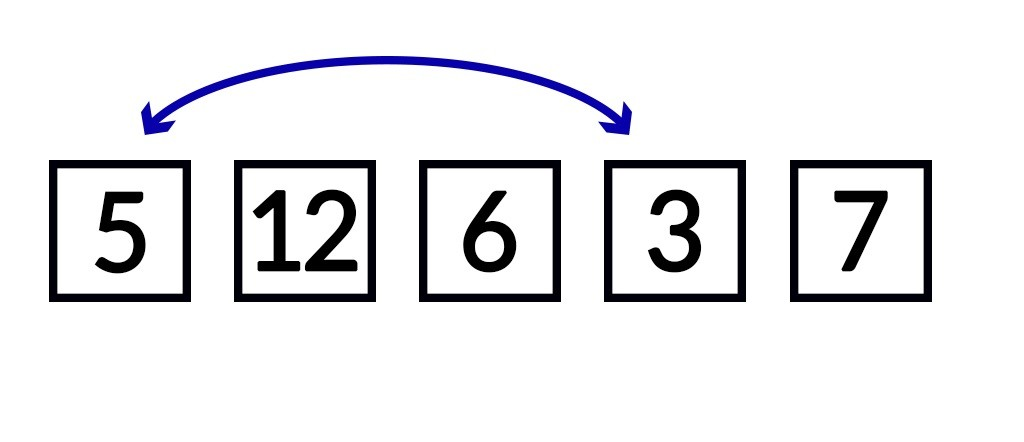
\includegraphics[width=5cm]{IMG_1125.JPG}
	\raggedright
	\paragraph{\color{blue}Materialien} \mbox{} \\
	\begin{itemize}
		\item mind. 2 Blätter A4-Papier mit unterschiedlichen Nummern bedruckt.
	\end{itemize}
	
	\raggedright
	\paragraph{\color{blue}Anleitung} \mbox{} \\
	\begin{enumerate}
		\item Jeder Schüler erhält ein Blatt
		\item Die Schüler stellen sich in einer unsortierten Reihenfolge auf.
		\item Es wird sich für einen Sortieralgorithmus entschieden.
		\item Die Schritte des gewählten Algorithmuses werden nacheinander durchgeführt, bis die Schüler in der sortierten Reihenfolge stehen.
	\end{enumerate}
	
	\raggedright
	\paragraph{\color{blue}Erklärung} \mbox{} \\
	
	Ein Algorithmus ist eine Reihenfolge von Anweisungen, die zu einem gewissen Ziel führen.
	Dieser kann dazu verwendet werden ein gewisses Problem zu lösen.
	Ein Sortieralgorithmus ist, wie der Name schon sagt, dafür da, eine Datenmenge in die richtige Reihenfolge zu bringen.
	Es gibt verschiedene Sortieralgorithmen, die unterschiedlich schnell bzw. effizient sind. Ein sehr einfacher Algorithmus ist der Bubble-Sort-Algorithmus. 	\newpage
	
	\thispagestyle{empty}
	
	\bslinespacing{1.5}
	{
		\centering
		\Huge
		\color{blue}
		Magnetflitzer
	}
	
	\centering
	\raggedright
	\paragraph{\color{blue}Materialien} \mbox{} \\
	\begin{itemize}
		\item Für den Magnetflitzer wird ein etwa 10 Meter langer Kupferdraht benötigt.
		Dieser sollte einen Durchmesser von 0.8cm besitzen.
		\item Ebenfalls benötigt wird eine Batterie (am besten funktionieren Varta Batterien mit 1.5V)
		\item Es werden 4 Neodym-Magnete benötigt. 
	\end{itemize}
	\paragraph{\color{blue}Anleitung} \mbox{} \\
	\begin{enumerate}
		\item Der Kupferdraht wird zu einer Spule gedreht, welche idealerweise einen Durchmesser von etwa 1,7cm aufweisen.
		\item Bei Bedarf kann die Spule gekürzt oder erweitert werden, um eine längere bzw. kürzere Strecke herzustellen.
		\item An den beiden Polen der Batterie müssen jeweils 2 Magnete befestigt werden.
		\item Abschließend wird die Batterie in die Spule eingeführt. Sollte sie sich nicht bewegen, muss die Polung der Magnete an der Batterie solange geändert werden, bis sie sich bewegt.
	\end{enumerate}
	Der Boden unter der Spule sollte möglichst glatt sein. 
	Besonders Pappe eignet sich als Unterlage.
	
	
\end{document}